\section{Design}
The concept for the GeoLog originally came from Dr. Andrew D. Wickert (seen in figure 
\ref{fig:andrewWickert}), which came to Reykjavík University's Mechatronics class for 
help developing his design of a low cost, low power datalogger\cite{ALog-BottleLogger}. 
He had two problems needed to be solved. First was to minimize the power consumption of the device he had already developed and the latter was to have means of getting the data
back without having to travel trough difficult terrain. Decision was made to help Andrew 
improve the latter with emphasis on making the system as modular as possible. 

\begin{figure}
\centering
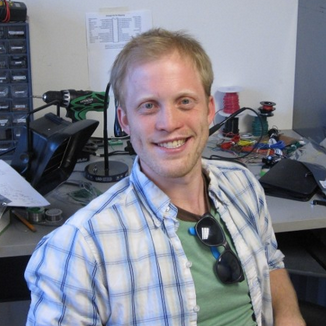
\includegraphics[width=0.4\linewidth]{graphics/andrewWickert}
\caption{Andrew Wickert\label{fig:andrewWickert}\cite{andrewWickert}}
\end{figure}

The GeoLog datalogger was designed in nine phases. Phases seven to eight were iterated
until the product was ready for deployment.

\begin{itemize}
    \item{Phase 1:} Initial brainstorming and high level design phase.
    \item{Phase 2:} Hardware selection phase, where hardware was selected and ordered.
    \item{Phase 3:} Software design phase, where the classes and interfaces were designed.
    \item{Phase 4:} Hardware hacking phase, trial and error in software writing for the
                    Wixels\cite{wixel} and the GSM/GPRS module\cite{SM5100B}.
    \item{Phase 5:} Building phase, where hardware were assembled.
    \item{Phase 6:} Software integration phase, all the software integrated to one.
    \item{Phase 7:} Field testing phase, testing of the system in real life environment.
    \item{Phase 8:} Fixing phase, fixing bugs found in the field testing phase.
    \item{Phase 9:} Deployment phase, system is functional and can be deployed. 
\end{itemize}

\textit{\textcolor{red}{Assumptions stated (There are always some)}}


\subsection{Hardware}
\begin{figure}
\centering
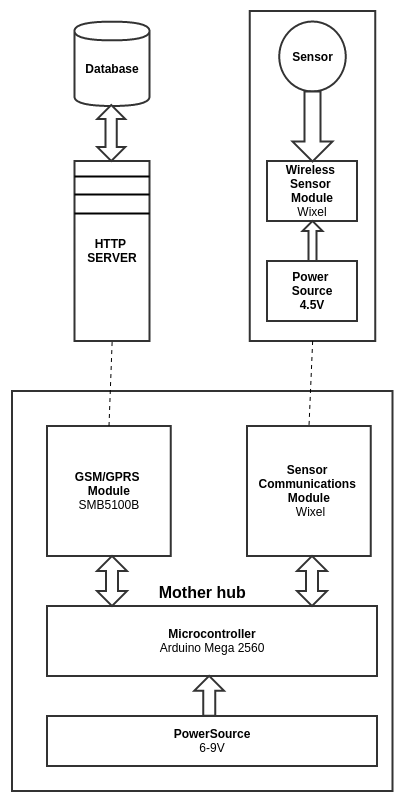
\includegraphics[width=0.5\linewidth]{graphics/HardwareMDD}
\caption{Hardware Module Design Diagram\label{fig:HardwareMDD}}
\end{figure}

The hardware is divided to sensor modules and the mother hub. The sensor modules 
designed for this system were three wireless temperature sensors using Wixel\cite{wixel}
for means of communications. The mother hub consists of a Arduino Mega\cite{arduinoMega}
that communicates with the sensor modules with a Wixel, collects the data 
and sends it to a HTTP server via the GSM/GPRS module\cite{SM5100B}. 
Figure \ref{fig:HardwareMDD} shows how the hardware is set up. 

\subsubsection{Sensor module}
The sensor module is based on Wixel\cite{wixel} that reads sensor value on one of it's
analog inputs when the mother hub calls for reading. To save energy the sensor module does
not send any data until it's id is called by the mother hub. The sensor module then 
gathers several readings from the sensor over a short period of time and sends back the 
average reading of the data collected then falls back to suspend mode until the mother 
hub calls for data again. Electrical schematic diagram of the sensor module can
be seen in figure \ref{fig:sensormodule_schematic}.

\subsubsection{Mother hub}
The mother hub is based on Arduino Mega 2560\cite{arduinoMega} which can be switched out 
for Andrew's Bottle Logger\cite{ALog-BottleLogger}, a Wixel\cite{wixel} used for 
communicating with the wireless sensor modules and a SM5100B GSM/GPRS 
module\cite{SM5100B}. The mother hub gathers data from the Wireless sensor modules via 
the onboard Wixel by calling them by id and wait till corresponding sensor module answers
with newly gathered sensor data. The data gathered is then saved to its onboard EEPROM
and at a preset time the data is sent to HTTP server via GPRS where it can be processed 
by the researcher. Electrical schematic diagram of the mother hub can be seen in figure 
\ref{fig:motherhub_schematic}.

\subsection{Software}
\begin{figure}
\centering
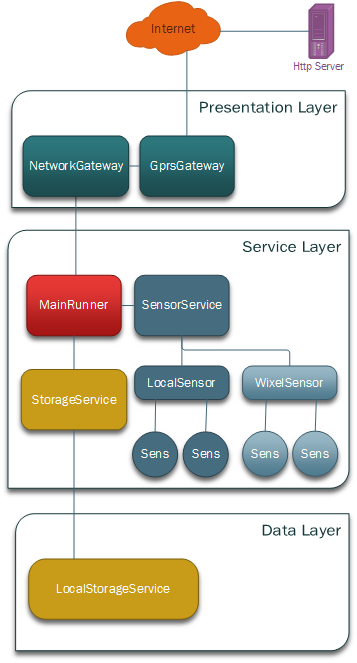
\includegraphics[width=0.6\linewidth]{graphics/Layering}
\caption{Layered Design Diagram of the system\label{fig:Layering}}
\end{figure}

When designing the software, modularity was the main interest. The design aims for making
it as easy as possible to implement new ways of communications, sensors and storage. This 
is done by building the software up of three interfaces the user needs to implement if for
example another means of communications is needed. The system comes with two ways of
communications to the outside world, a SMS gateway and a GPRS HTTP gateway. It comes also with one way of storing data, to the EEPROM and one way of communicating to wireless sensors. Figure \ref{fig:Layering} shows the layered design of the software. 

To take a closer look in to the software and how the interfaces work see the class diagram
shown in figure \ref{fig:ClassDiagram}. Next sections will describe more thoroughly how each 
module works under the hood. All code is written in C++ except the HTTP server which is 
written in Python/Flask-Restful.

\subsubsection{Sensor Service interface}
The sensor service is a interface the developer needs to implement for every new kind of
sensor module. The sensor service interface has three virtual methods that the developer
needs to implement by inheriting from the SensorService class.The methods needing implementation are the following:
\begin{itemize}
    \item \textbf{int getSensorData(int sensorId)}
        \begin{itemize}
            \item Takes in the id of the sensor and returns the raw value.
        \end{itemize}
    \item \textbf{int sendDataToSensor(String data)}
        \begin{itemize}
            \item Takes in data to send to sensor and returns 0 for OK and -1 for error.
                  This could be used to remote calibrate sensor.
        \end{itemize}
    \item \textbf{int setDateTime(long DateTime)}
        \begin{itemize}
            \item Takes in UNIX date/time for setting the time on the sensor if needed.
        \end{itemize}
\end{itemize}
The Sensor service now implemented is the WixelSensorService. This service communicates 
with the Wixel Sensor Modules, converts the raw data to a value of interest like 
temperature and finally parses the converted data to Json\cite{json} strings. Sample
of Json parsed data can be seen in figure \ref{fig:JsonTemp}. Pseudocode of the 
getSensorData method can be seen in listing \ref{pseodoWixelSensorService}.


\begin{lstlisting}[frame=single, label=pseodoWixelSensorService, caption={Pseudocode of WixelSensorService getSensorData() function}]
Function(getSensorData(sensorId)):
    define wixelSerialPort as desired serial port
    define TimeOut as desired timeout in milliseconds
    define startTime as current time in milliseconds
    define data as 0;
    while data equals 0 or ((current time - startTime) > TimeOut:
        write sensorId to wixelSerialPort
        wait for 100 milliseconds
        if wixelSerialPort read buffer is not empty:
            data = data read from wixelSerialPort
            flush wixelSerialPort
        end if
    end while
    return data converted to celsius
end Function(getSensorData)
\end{lstlisting}

\begin{figure}
\centering
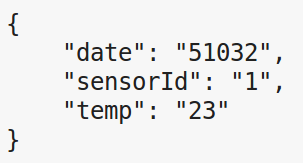
\includegraphics{graphics/JsonTemp}
\caption{Json\cite{json} string received from the WixelSensorService\label{fig:JsonTemp}}
\end{figure}

\subsubsection{Storage Service interface}
The storage service is a interface the developer needs to implement if a new way of
storing data is needed. The storage service interface has four virtual methods that the developer needs to implement by inheriting from the StorageService class. The methods needing implementation are the following:
\begin{itemize}
    \item \textbf{int save(String data)}
        \begin{itemize}
            \item Takes in data in String format and saves it to storage medium. 
                  Returns number of bytes saved, returns -1 if not enough space.
        \end{itemize}
    \item \textbf{String load()}
        \begin{itemize}
            \item Loads all data in memory and returns it in string format.
        \end{itemize}
    \item \textbf{int erase()}
        \begin{itemize}
            \item Erases all data from storage medium. Returns number of bytes
                  free after erase.
        \end{itemize}
    \item \textbf{bool isFreeSpcace(int dataSize)}
        \begin{itemize}
            \item Takes in size of data to be saved in bytes. Returns true if enough 
                  space is available, false if not.
        \end{itemize}
\end{itemize}
The Storage Service now implemented is the LocalStorageService. This service stores data 
to the Arduino's EEPROM. The Arduino Mega 2560 has 4096 bytes of 
EEPROM \cite{arduinoMega}. The LocalStorageService stores the data as series of Json 
strings. A typical use of the LocalStorageService is first to use the isFreeSpace() method
to check if enough space is available for the data to be stored. If space is enough the save() method is used to save the data to the EEPROM. If space is not available the developer has to take some action like loading all existing data using the load() method, send the data to the HTTP server before using the erase() function to erase the EEPROM for new data. Pseudocode of the save(), load() and erase() methods can be seen in 
listings \ref{pseodoLocalStorageService}

\begin{lstlisting}[frame=single, label=pseodoLocalStorageService, caption={Pseudocode of LocalStorageService save(), load() and erase() functions}]
Function(save(data)):
    define iterator as 0
    define i = 0
    for i < EEPROM size:
        read byte i from EEPROM
        if byte i equals 0:
            break
        end if
        iterator = iterator + 1
        i = i + 1
    end for
    if not enough space for data:
        return -1
    else:
        define dataSize as 0
        define j as 0
        for j < data size in bytes:
            if iterator >= (EEPROM size -1):
                break
            end if
            write byte at index j in data to EEPROM address that equals iterator
            iterator = iterator + 1
            dataSize = dataSize +1
        end for
        write ',' to EEPROM address corresponding to iterator
        dataSize = dataSize + 1
        return dataSize
    end if
end Function(save(data))

Function(load):
    define data as string
    define i as 0
    define letter
    for i < EEPROM size:
        letter = byte at EEPROM address that equals i
        if letter equals 0:
            break
        end if
        append letter to data
    end for
    return data
end Function(load)

Function(erase):
    define counter as 0
    define i as 0
    for < EEPROM size:
        counter = counter + 1
        write 0 to EEPROM address that equals i
    end for
    if counter not equals EEPROM size:
        return -1
    else:
        return counter
    end if
Function(erase)
\end{lstlisting}
\subsubsection{Network Gateway interface}

\begin{itemize}
    \item \textbf{bool connectToNetwork()}
        \begin{itemize}
            \item Connects to network. Returns true if connected, false if not
                  connected to network.
        \end{itemize}
    \item \textbf{bool connected()}
        \begin{itemize}
            \item Checks if connected to network. Returns true if connected, false
                  if not connected.
        \end{itemize}
    \item \textbf{int sendData(String address, String data)}
        \begin{itemize}
            \item Sends given data to given address. Returns number of bytes sent, -1 if 
                  error sending data.
        \end{itemize}
    \item \textbf{String reciveData(String address)}
        \begin{itemize}
            \item Gets data from given address. Returns the data.
        \end{itemize}
     \item \textbf{long getTime()}
        \begin{itemize}
            \item Gets the current time/date from the network. Returns the time in UNIX time/date as long.
        \end{itemize}
\end{itemize}

\subsubsection{Main Runner}

\subsubsection{HTTP Server}

\textit{\textcolor{red}{Description of the design; break into pieces and show how 
                        they assemble.}}

\textit{\textcolor{red}{Pseudo code of important modules}}

\textit{\textcolor{red}{MDD of structure}}

\textit{\textcolor{red}{System diagram}}

\subsection{Safety}
